\section{Similarità del coseno}
Lo spazio latente di un LLM è un ambiente vettoriale ad alta dimensionalità, superiore a 4000 dimensioni, all'interno del quale le relazioni semantiche obbediscono a leggi geometriche. Uno degli obiettivi cardine di questo studio è verificare l'esistenza di un allineamento geometrico, ovvero il grado di congruenza geometrica, tra le perturbazioni indotte dagli attacchi testuali Black-Box e la direzione pura della vulnerabilità calcolata matematicamente White-Box.

Il termine di paragone per questa indagine è il Vettore di Steering. Come descritto nel Capitolo 5, questo vettore rappresenta l'asse semantico naturale del modello, calcolato come differenza tra i centroidi dei codici sicuri e vulnerabili. 
L'operazione si articola in tre fasi computazionali distinte:\\

\textbf{FASE 1: Estrazione degli Stati Latenti}\\
Per garantire un paragone geometricamente puro, l'estrazione non viene limitata all'output testuale, bensì sfrutta il parametro output\_hidden\_states=True di PyTorch per estrarre la precisa mappa delle sue attivazioni interne nel forward pass.
Per ciascun codice vulnerabile del dataset, il modello viene sottoposto a due iterazioni di inferenza:
\begin{itemize}[noitemsep]
    \item Inferenza di Riferimento: Il codice originariamente identificato come vulnerabile viene processato, registrando la traiettoria latente originale del modello.
    \item Inferenza Attaccata: Lo stesso codice, ma con perturbazione testuale, viene processato dal modello.
\end{itemize}

In entrambe le fasi, viene estratta l'attivazione vettoriale corrispondente all'esatto istante precedente la generazione finale, momento di massima densità informativa per il verdetto nonché l'ultimo token della sequenza in input.\\

\textbf{FASE 2: Calcolo dello Shift Vettoriale Individuale}\\
Una volta estratti gli hidden states per ogni livello dell'architettura del modello, viene calcolato lo \textit{Shift Vettoriale}, definito come la differenza vettoriale tra lo stato latente attaccato e lo stato di riferimento pulito:
\begin{equation}
\Delta V_L = h_{L,\text{attacco}} - h_{L,\text{pulito}}
\end{equation}
Questo vettore differenza rappresenta la pura direzione generata dall'attacco per quel singolo frammento di codice.

\begin{minted}[linenos, frame=lines, framesep=2mm, fontsize=\footnotesize, breaklines]{python}
    
def get_all_hidden_states(codice):
            prompt = f"Analyze this code \n\nCode:\n{codice}, \n start the response EXACTLY with 'FINAL_VERDICT: True' (if vulnerable) or 'FINAL_VERDICT: False' (if 100% secure), followed by a brief summary."
            messages = [{"role": "system", "content": "You are a cybersecurity expert. Your task is to find vulnerabilities in the source code."}, {"role": "user", "content": prompt}]
            testo = tokenizer.apply_chat_template(messages, tokenize=False, add_generation_prompt=True)
            inputs = tokenizer([testo], return_tensors="pt").to(model.device)
            with torch.no_grad():
                out = model(**inputs, output_hidden_states=True)
            return torch.stack([layer_state[0, -1, :] for layer_state in out.hidden_states])

        for index, row in df_mod.iterrows():
            codice_pulito = str(row['codice_originale']) 
            codice_hackerato = str(row['codice_perturbato'])

            h_clean = get_all_hidden_states(codice_pulito)
            h_adv = get_all_hidden_states(codice_hackerato)
            shift_all = h_adv - h_clean

            for layer_idx in range(num_layers_totali):
                vettore_riferimento = dizionario_vettori[layer_idx]
                if vettore_riferimento is not None:
                    shift_layer = shift_all[layer_idx]
                    cos_sim = F.cosine_similarity(shift_layer, vettore_riferimento, dim=0).item()
                    accumulatore_sim[layer_idx].append(cos_sim)
        
\end{minted}


\textbf{FASE 3: Calcolo della similarità del coseno}\\
Dopo aver calcolato lo shift direzionale del vettore dell'attacco Black-Box, viene eseguita la cosine similarity tra tutti i codici in cui l'attacco ha avuto successo e il vettore di steering. \\
La \textit{Cosine Similarity}, o similarità del coseno, è una metrica matematica utilizzata per misurare quanto due vettori sono simili tra loro in uno spazio multidimensionale. Infatti, calcola il coseno dell'angolo compreso tra due vettori valutandone l'orientamento ed ignorando la loro lunghezza.
L'equazione è definita come:

\begin{equation}
    \text{Cosine Similarity} = cos(\theta) = \frac{A \cdot B}{||A|| ~~ ||B||}
\end{equation}



\begin{itemize}[noitemsep]
    \item \textit{Il Numeratore $(A\cdot B)$}: È il prodotto scalare tra i due vettori: se vanno nella stessa direzione, questo numero cresce; se vanno in direzioni opposte, diventa negativo.
    \item \textit{Il Denominatore ($||A|| \cdot ||B||$)}: È il prodotto delle magnitudini, ovvero la lunghezza dei due vettori. 
\end{itemize}
Dividendo il prodotto scalare per le lunghezze l'equazione viene normalizzata in modo tale che, indipendentemente dalla lunghezza del vettore, ciò che verrà preso in esame sarà solo l'angolo tra i due vettori.

L'uso della cosine similarity quindi permette di dire l'angolazione di un vettore rispetto ad un altro, indicando quanto questi siano simili: vettori semanticamente simili saranno paralleli, ottenendo una Cosine Similarity di $1$ o $-1$ a seconda del verso. Al contrario, vettori rappresentanti concetti semantici completamente incongruenti o scorrelati risulteranno ortogonali nello spazio ad alta dimensionalità, restituendo un valore prossimo allo $0$.
Invece di calcolare un singolo vettore medio, che rischierebbe di annullare le direzioni divergenti, viene calcolata la media per ogni attacco avvenuto con successo di tutti gli angoli ottenuti.


\begin{table}[H]
    \centering
    \begin{tabular}{l c c c}
        \toprule
        \textbf{Modelli} & \textbf{Cosine Similarity} & \textbf{Angolo} & \textbf{N. Successi}\\
        \midrule
        Qwen/Qwen2.5-7B-Instruct                 & 0.176  & 79.86$^\circ$ & 91 \\
        Qwen/Qwen2.5-Coder-7B-Instruct           & 0.144  & 81.72$^\circ$ & 75 \\
        meta-llama/Llama-3.1-8B-Instruct         & 0.318  & 71.46$^\circ$ & 1 \\
        codellama/CodeLlama-7b-Instruct-hf       & 0.554  & 56.36$^\circ$ & 6 \\
        deepseek-ai/DeepSeek-R1-Distill-Qwen-7B  & 0.060  & 86.56$^\circ$ & 46 \\
        deepseek-ai/deepseek-coder-6.7b-instruct & 0.114  & 83.45$^\circ$ & 5 \\
        \bottomrule
    \end{tabular}
    \vspace{0.2cm}
    \caption{Esito similarità tra attacco Advanced Adversarial e Steering Vector sul weakest layer}
    \label{tab:esito_iso_AA}
\end{table}


\begin{table}[H]
    \centering
    \begin{tabular}{l c c c}
        \toprule
        \textbf{Modelli} & \textbf{Cosine Similarity} & \textbf{Angolo} & \textbf{N. Successi} \\
        \midrule
        Qwen/Qwen2.5-7B-Instruct                 & 0.089  & 89.89$^\circ$ & 69 \\
        Qwen/Qwen2.5-Coder-7B-Instruct           & 0.068  & 86.10$^\circ$ & 63 \\
        meta-llama/Llama-3.1-8B-Instruct         & -      & -             & 0 \\
        codellama/CodeLlama-7b-Instruct-hf       & 0.365  & 68.59$^\circ$ & 26 \\
        deepseek-ai/DeepSeek-R1-Distill-Qwen-7B  & 0.033  & 88.11$^\circ$ & 115\\
        deepseek-ai/deepseek-coder-6.7b-instruct & 0.026  & 88.51$^\circ$ & 3 \\
        \bottomrule
    \end{tabular}
    \vspace{0.2cm}
    \caption{Esito similarità tra attacco Advanced Pertubration e Steering Vector sul weakest layer}
    \label{tab:esito_iso_AP}
\end{table}


\begin{table}[H]
    \centering
    \begin{tabular}{l c c c}
        \toprule
        \textbf{Modelli} & \textbf{Cosine Similarity} & \textbf{Angolo} & \textbf{N. Successi} \\
        \midrule
        Qwen/Qwen2.5-7B-Instruct                 & 0.076  & 85.64$^\circ$ & 88 \\
        Qwen/Qwen2.5-Coder-7B-Instruct           & 0.067  & 86.16$^\circ$ & 51 \\
        meta-llama/Llama-3.1-8B-Instruct         & -0.015 & 90.86$^\circ$ & 131\\
        codellama/CodeLlama-7b-Instruct-hf       & 0.146  & 81.61$^\circ$ & 199\\
        deepseek-ai/DeepSeek-R1-Distill-Qwen-7B  & 0.020  & 88.85$^\circ$ & 140\\
        deepseek-ai/deepseek-coder-6.7b-instruct & -0.115 & 96.60$^\circ$ & 1 \\
        \bottomrule
    \end{tabular}
    \vspace{0.2cm}
    \caption{Esito similarità tra attacco Prompt Injection e Steering Vector sul weakest layer}
    \label{tab:esito_iso_PI}
\end{table}

I risultati rivelano una dinamica spaziale fondamentale per la comprensione delle vulnerabilità dei Large Language Models. La Cosine Similarity media registrata è prossima allo zero, rispettivamente $0.231$, $0.128$ e $0.085$ per le tre classi di attacco Advanced Adversarial, Advanced Perturbation e Prompt Injection, indicando che i vettori rappresentanti gli attacchi formano angoli vicini ai $90^\circ$ rispetto al vettore di steering.

Ciò dimostra una quasi totale assenza di parallelismo di azione: gli attacchi Black-Box non ingannano il modello spingendolo lungo il naturale asse semantico che separa la vulnerabilità dalla sicurezza. Al contrario, le perturbazioni come l'inserimento di codice morto o istruzioni di override spingono l'elaborazione latente in dimensioni completamente ortogonali. Il modello non viene propriamente portato a pensare che il codice sia sicuro nel senso stretto, ma viene deragliato in una regione dello spazio vettoriale di confusione geometrica, dove i filtri di rilevamento delle minacce perdono la loro efficacia direzionale, portando la rete a collassare sul verdetto di baseline true/false.

\subsection{Similarità Black-Box}
Al fine di ottenere una panoramica più completa sulla similarità tra attacchi, viene eseguita l'analisi della cosine similarity tra i vettori degli attacchi Black-Box per verificare se esiste un parallelismo tra le modalità di attacco delle perturbazioni.
L'obiettivo è quindi verificare se è possibile posizionare gli attacchi su uno spettro delle direzioni di attacco.
Perché questo sia possibile viene effettuata l'indagine di cosine similarity sui codici che hanno avuto successo per entrambi gli attacchi, confrontando quindi i vettori a coppie di black-box invece che con il vettore di steering. 

\begin{table}[H]
    \centering
    \begin{tabular}{l c c }
        \toprule
        \textbf{Modelli} & \textbf{Cosine Similarity} & \textbf{Angolo} \\
        \midrule
        Qwen/Qwen2.5-7B-Instruct                 & 0.11  & 83.66$^\circ$ \\
        Qwen/Qwen2.5-Coder-7B-Instruct           & 0.249  & 75.56$^\circ$ \\
        meta-llama/Llama-3.1-8B-Instruct         & 0.133 & 82.38$^\circ$ \\
        codellama/CodeLlama-7b-Instruct-hf       & 0.360  & 68.89$^\circ$ \\
        deepseek-ai/DeepSeek-R1-Distill-Qwen-7B  & 0.232  & 76.57$^\circ$ \\
        deepseek-ai/deepseek-coder-6.7b-instruct & 0.138 & 82.04$^\circ$ \\
        \bottomrule
    \end{tabular}
    \vspace{0.2cm}
    \caption{Similarità tra Advanced Adversarial e Prompt Injection sul weakest layer}
    \label{tab:esito_iso_AA_PI}
\end{table}

\begin{table}[H]
    \centering
    \begin{tabular}{l c c }
        \toprule
        \textbf{Modelli} & \textbf{Cosine Similarity} & \textbf{Angolo} \\
        \midrule
        Qwen/Qwen2.5-7B-Instruct                 & 0.437  & 64.11$^\circ$ \\
        Qwen/Qwen2.5-Coder-7B-Instruct           & 0.567  & 55.47$^\circ$ \\
        meta-llama/Llama-3.1-8B-Instruct         & - & - \\
        codellama/CodeLlama-7b-Instruct-hf       & 0.621  & 51.62$^\circ$ \\
        deepseek-ai/DeepSeek-R1-Distill-Qwen-7B  & 0.637  & 50.45$^\circ$ \\
        deepseek-ai/deepseek-coder-6.7b-instruct & 0.605 & 52.78$^\circ$ \\
        \bottomrule
    \end{tabular}
    \vspace{0.2cm}
    \caption{Similarità tra Advanced Adversarial e Adversarial Perturbation sul weakest layer}
    \label{tab:esito_iso_AA_AP}
\end{table}

\begin{table}[H]
    \centering
    \begin{tabular}{l c c }
        \toprule
        \textbf{Modelli} & \textbf{Cosine Similarity} & \textbf{Angolo} \\
        \midrule
        Qwen/Qwen2.5-7B-Instruct                 & 0.184  & 79.38$^\circ$ \\
        Qwen/Qwen2.5-Coder-7B-Instruct           & 0.425  & 64.85$^\circ$ \\
        meta-llama/Llama-3.1-8B-Instruct         & - & - \\
        codellama/CodeLlama-7b-Instruct-hf       & 0.468  & 62.07$^\circ$ \\
        deepseek-ai/DeepSeek-R1-Distill-Qwen-7B  & 0.327  & 70.93$^\circ$ \\
        deepseek-ai/deepseek-coder-6.7b-instruct & 0.337 & 70.29$^\circ$ \\
        \bottomrule
    \end{tabular}
    \vspace{0.2cm}
    \caption{Similarità tra Adversarial Perturbation e Prompt Injection sul weakest layer}
    \label{tab:esito_iso_AP_PI}
\end{table}


I risultati mostrano risultati diversi rispetto a quanto ottenuto con la cosine similarity con il vettore di steering:

\begin{itemize}[noitemsep]
    \item Advanced Adversarial e Prompt Injection: 0.20 (78.46$^\circ$)
    \item Advanced Adversarial e Adversarial Perturbation: 0.57 (55.25$^\circ$)
    \item Adversarial Perturbation e Prompt Injection: 0.35 (69.51$^\circ$)
\end{itemize}

Considerando l'alta dimensionalità in cui vengono posizionati i vettori, le perturbazioni di Advanced Adversarial e Adversarial Pertubration dimostrano avere un valore di cosine similarity molto alto di $0.57$, evidenziando un alta somiglianza tra le metodologie dei due attacchi.
Prompt Injection e Adversarial Pertubration hanno un valore di circa 0.37, mentre Advanced Adversarial e Prompt Injection di 0.25. Questi valori indicano una discreta somiglianza non del tutto trascurabile di questi attacchi: nonostante l'angolazione non sia parallela sono numeri maggiori rispetto allo steering.
Le motivazioni di questi valori risiedono nelle metodologie degli attacchi stessi: gli attacchi Advanced Adversarial e Adversarial Perturbation lavorano entrambi sul codice offuscando variabili, aggiungendo codice morto o alterando la sintassi, rimanendo all'interno della logica di programmazione.
Prompt Injection è invece diverso: non offusca il codice ma inietta un comando diretto lavorando sull'ubbidienza e non sulla sintassi, ponendosi quindi distante dagli altri due.
Si può quindi ipotizzare l'esistenza di uno spettro su cui si collocano gli attacchi Black-Box considerando ad un estremo la perturbazione con la media più bassa, Prompt Injection, per poi collocare in sequenza gli attacchi di Adversarial Perturbation e Advanced Adversarial.

Tutti questi attacchi, tuttavia, condividono una caratteristica fondamentale scoperta nella fase precedente: nessuno di essi riesce a replicare la pura traiettoria vettoriale della vulnerabilità dello steering vector confermando come gli attacchi testuali si configurano come deviazioni ortogonali che fanno smarrire la rete nello spazio latente.

A riprova di quanto affermato è stato eseguito il calcolo della cosine similarity anche per gli attacchi falliti ottenendo i seguenti risultati sul weakest layer:

\begin{table}[H]
    \centering
    \begin{tabular}{l c c c}
        \toprule
        \textbf{Modelli} & \textbf{AA} & \textbf{AP} & \textbf{PI}\\
        \midrule
        Qwen/Qwen2.5-7B-Instruct                 & 0.179  & 0.094 & 0.102 \\
        Qwen/Qwen2.5-Coder-7B-Instruct           & 0.143  & 0.123 & 0.090 \\
        meta-llama/Llama-3.1-8B-Instruct         & 0.216  & 0.140 & -0.030 \\
        codellama/CodeLlama-7b-Instruct-hf       & 0.497  & 0.354 & - \\
        deepseek-ai/DeepSeek-R1-Distill-Qwen-7B  & 0.047  & 0.022 & 0.012\\
        deepseek-ai/deepseek-coder-6.7b-instruct & -0.038  & 0.062 & 0.041 \\
        \bottomrule
    \end{tabular}
    \vspace{0.2cm}
    \caption{Esito cosine similarity tra attacchi falliti e vettore di steering}
    \label{tab:esito_iso_vuln}
\end{table}

\begin{table}[H]
    \centering
    \begin{tabular}{l c c c}
        \toprule
        \textbf{Modelli} & \textbf{AA e AP} & \textbf{AA e PI} & \textbf{AP e PI}\\
        \midrule
        Qwen/Qwen2.5-7B-Instruct                 & 0.389  & 0.160 & 0.003 \\
        Qwen/Qwen2.5-Coder-7B-Instruct           & 0.539  & 0.238 & 0.516 \\
        meta-llama/Llama-3.1-8B-Instruct         & 0.582  & 0.017 & 0.388 \\
        codellama/CodeLlama-7b-Instruct-hf       & 0.711  & - & - \\
        deepseek-ai/DeepSeek-R1-Distill-Qwen-7B  & 0.613  & 0.226 & 0.363\\
        deepseek-ai/deepseek-coder-6.7b-instruct & 0.397  & 0.274 & 0.410 \\
        \bottomrule
    \end{tabular}
    \vspace{0.2cm}
    \caption{Esito cosine similarity tra attacchi falliti}
    \label{tab:esito_iso_vuln2}
\end{table}

Come si può osservare dagli esiti presenti nella tabella \ref{tab:esito_iso_vuln}, viene riconfermato come gli attacchi Black-Box operino in modo quasi del tutto perpendicolare rispetto al vettore di steering, presentando una cosine similarity molto bassa ad eccezione del modello CodeLlama.
I risultati ottenuti dalla cosine similarity tra attacchi evidenziano ancora di più quanto affermato nella prima analisi: Advanced Adversarial e Adversarial Perturbation riportano una cosine similarity molto alta, sottolineando come i meccanismi dietro questi attacchi sia estremamente simile e operi cercando di portare il modello nella stessa area dello spazio latente.

Sia per gli attacchi riusciti che per quelli falliti, il valore di cosine similarity è vicino al numero calcolato sul weakest layer, con leggere fluttuazioni che però non evidenziano grosse implicazioni rispetto a quanto esposto precedentemente.

\begin{figure}[H]
    \centering
    
    \begin{subfigure}[b]{0.45\textwidth}
        \centering
        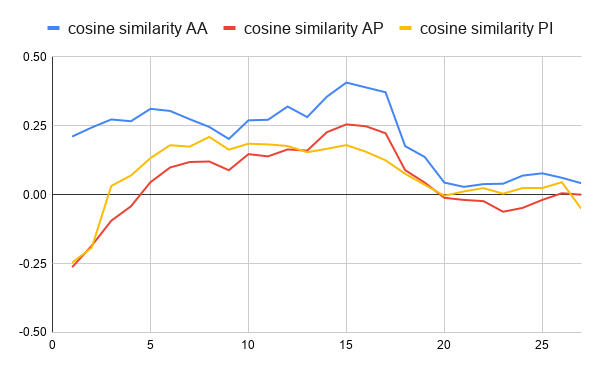
\includegraphics[width=\textwidth]{immagini/iso_es.png} 
        \caption*{Qwen2.5-7B-Instruct}
        \label{fig:iso_es}
    \end{subfigure}
    \hfill 
    \begin{subfigure}[b]{0.45\textwidth}
        \centering
        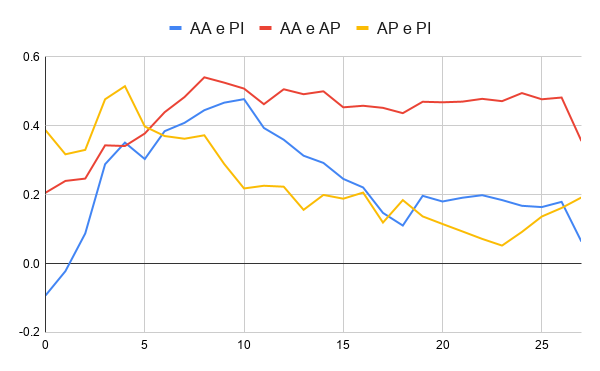
\includegraphics[width=\textwidth]{immagini/iso_es2.png} 
        \caption*{Qwen2.5-7B-Instruct Black-Box}
        \label{fig:iso_es2}
    \end{subfigure}
    
    \vspace{0.2cm}
    \caption{Similarità sweep attacchi riusciti}
    \label{fig:iso_es3}
\end{figure}

\begin{figure}[H]
    \centering
    
    \begin{subfigure}[b]{0.45\textwidth}
        \centering
        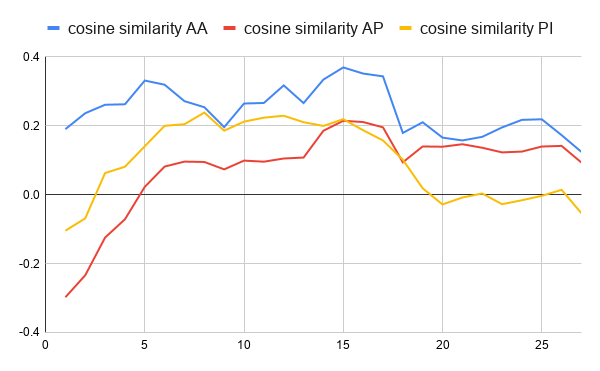
\includegraphics[width=\textwidth]{immagini/iso_vuln_bb.png} 
        \caption*{Qwen2.5-7B-Instruct}
        \label{fig:iso_ess}
    \end{subfigure}
    \hfill 
    \begin{subfigure}[b]{0.45\textwidth}
        \centering
        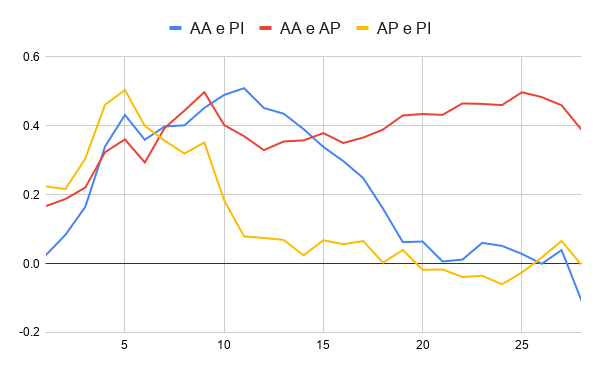
\includegraphics[width=\textwidth]{immagini/iso_vuln_comp.png} 
        \caption*{Qwen2.5-7B-Instruct Black-Box}
        \label{fig:iso_ess2}
    \end{subfigure}
    
    \vspace{0.2cm}
    \caption{Similarità sweep attacchi falliti}
    \label{fig:iso_ess3}
\end{figure}

Si può osservare come solo gli attacchi più simili meccanicamente, quali Advanced Adversarial e Adversarial Perturbation, mantengano un valore di cosine similarity alto in quasi la totalità dei layer a differenza delle altre perturbazioni che mostrano un andamento disomogeneo.
Al fine di avere una visione più completa vengono presentati i picchi massimi ottenuti nei layer.

\begin{table}[H]
    \centering
    \begin{tabular}{l c c c c c c}
        \toprule
        \textbf{Modelli} & \textbf{AA} & \textbf{AP} & \textbf{PI} & \textbf{AA e AP} & \textbf{AA e PI} & \textbf{AP e PI}\\
        \midrule
        Qwen2.5-7B-Instruct                 & 0.407 & 0.255 & 0.210 & 0.541 & 0.477 & 0.515 \\
        Qwen2.5-Coder-7B-Instruct           & 0.448 & 0.345 & 0.369 & 0.612 & 0.515 & 0.559 \\
        Llama-3.1-8B-Instruct         & 0.680 & -     & 0.353 & -     & 0.599 & - \\
        CodeLlama-7b-Instruct-hf       & 0.608 & 0.401 & 0.178 & 0.750 & 0.406 & 0.544 \\
        DeepSeek-R1-Distill-Qwen-7B  & 0.196 & 0.108 & 0.231 & 0.685 & 0.236 & 0.569 \\
        deepseek-coder-6.7b-instruct & 0.213 & 0.198 & 0.096 & 0.659 & 0.297 & 0.507 \\
        \bottomrule
    \end{tabular}
    \vspace{0.2cm}
    \caption{Picchi massimi cosine similarity attacchi riusciti}
    \label{tab:esitone1}
\end{table}

\begin{table}[H]
    \centering
    \begin{tabular}{l c c c c c c}
        \toprule
        \textbf{Modelli} & \textbf{AA} & \textbf{AP} & \textbf{PI} & \textbf{AA e AP} & \textbf{AA e PI} & \textbf{AP e PI}\\
        \midrule
        Qwen2.5-7B-Instruct                 & 0.369 & 0.215 & 0.238 & 0.498 & 0.509 & 0.504 \\
        Qwen2.5-Coder-7B-Instruct           & 0.366 & 0.363 & 0.374 & 0.594 & 0.570 & 0.572 \\
        Llama-3.1-8B-Instruct         & 0.405 & 0.354 & 0.279 & 0.688 & 0.502 & 0.621 \\
        CodeLlama-7b-Instruct-hf       & 0.522 & 0.384 & -     & 0.711 & -     & -     \\
        DeepSeek-R1-Distill-Qwen-7B  & 0.190 & 0.097 & 0.234 & 0.684 & 0.257 & 0.587 \\
        deepseek-coder-6.7b-instruct & 0.249 & 0.138 & 0.114 & 0.601 & 0.331 & 0.584 \\
        \bottomrule
    \end{tabular}
    \vspace{0.2cm}
    \caption{Picchi massimi cosine similarity attacchi falliti}
    \label{tab:esitone2}
\end{table}